\documentclass[orivec]{llncs}
\usepackage{graphicx}
\usepackage{amsmath}			% for "cases"
\usepackage{amsfonts}		% for frakur fonts
\usepackage{mathrsfs}		% for curly "E" error symbol
\usepackage{float}
\usepackage{tcolorbox}		% for wrapping example in color box
\usepackage{wrapfig}			% wrap figure beside text, used in example
\usepackage{tikz-cd}			% commutative diagrams
\usepackage{amssymb}			% for \multimap, \updownarrow, \bigstar
\usepackage{sectsty}			% change section color
\usepackage{turnstile}		% longer turnstiles
\usepackage{hyperref}		% include web link for RL sample code

\usepackage{geometry}		% change paper size
\geometry{
  a4paper,         % or letterpaper
  textwidth=18cm,  % llncs has 12.2cm
  textheight=27cm, % llncs has 19.3cm
  heightrounded,   % integer number of lines
  hratio=1:1,      % horizontally centered
  vratio=2:3,      % not vertically centered
}
\usepackage[fontsize=13pt]{scrextend}

% *************** Delete when not using Chinese or colors **********************
\usepackage{xeCJK}
\setCJKmainfont[BoldFont=SimHei,ItalicFont=KaiTi]{SimSun}
\usepackage{color}
\definecolor{Cerulean}{RGB}{100,100,200}
\newcommand{\emp}[1]{\textbf{\textcolor{Cerulean}{#1}}}
\definecolor{grey}{rgb}{0.9,0.9,0.9}  % grey

% \chapterfont{\color{blue}}  % sets colour of chapters
\sectionfont{\color{blue}} 
\subsectionfont{\color{blue}} 
\subsubsectionfont{\color{blue}} 

\newcommand{\vect}[1]{\boldsymbol{#1}}
\newcommand*\sigmoid{\vcenter{\hbox{
\includegraphics{sigmoid.png}}}}
\newcommand*\KB{\vcenter{\hbox{
\includegraphics{KB-symbol.png}}}}
\newcommand*\invsigmoid{\vcenter{\hbox{
\includegraphics{inverse-sigmoid.png}}}}
\newcommand{\invW}{\, \rotatebox[origin=c]{90}{W}}
\newcommand{\invw}{\, \rotatebox[origin=c]{90}{w}}
\newcommand*\rectifier{\vcenter{\hbox{
\includegraphics{rectifier.png}}}}
\newcommand{\dashh}{\textemdash~}
\newcommand{\code}[1]{{\footnotesize{\ttfamily #1}}}
\newcommand{\tab}{\hspace*{1cm} }

% ***** Boxed variables inside math equations
% \newcommand*{\boxedcolor}{black}
\makeatletter
% \renewcommand{\boxed}[1]{\textcolor{\boxedcolor}{%
% \fbox{\normalcolor\m@th$\displaystyle#1$}}}
% \setlength{\fboxsep}{1pt}
\renewcommand{\boxed}[1]{\fbox{\m@th$\displaystyle\scalebox{0.9}{#1}$} \,}
\makeatother

\overfullrule=0mm

\newsavebox{\MyName}
\savebox{\MyName}{
\includegraphics[scale=0.6]{YKY.png}}

\title{游荡在思考的迷宫中}
\titlerunning{游荡在思考的迷宫中}
\author{\usebox{\MyName} (King-Yin Yan)
% \\ \footnotesize{General.Intelligence@Gmail.com}
% \and
% Juan Carlos Kuri Pinto
}
\institute{General.Intelligence@Gmail.com}

\begin{document}

\maketitle
\setlength{\parindent}{0em}
% \setlength{\parskip}{2.8ex plus0.8ex minus0.8ex}
\setlength{\parskip}{2.8ex}

\begin{abstract}
介绍一个基於 \textbf{增强学习} 和 \textbf{深度学习} 的极简约的 cognitive architecture,它在数学上是一个Hamiltonian 系统,而其 Lagrangian 对应於智能系统的「奖励」或「desire 的价值」。 经典逻辑 AI 的技巧可以搬到这个 setting 之下,而连续时间化之后,可以用上微分几何的技巧。 
% 简单介绍笔者的强人工智能理论和强化学习、动态规划、最优控制、
% 假设 $x$ 是思维状态。 在经典逻辑智能中,$x$ 是一束命题,代表当下的思考状况。 思考的过程就是不断重复进行推导: $x \vdash x' \vdash ...$。 在经典 AI 中这个作用是靠无数的逻辑 rules 来达成的。 但现在我们的做法是将 $x$ 放到向量空间中,再用一个 recurrent 神经网络来取代整个 rules base。
\end{abstract}

本文较少原创内容,主要介绍一些已知的理论,及提供一个新的观点,或许对 strong AI 的发展有帮助。

\section{中心思想}

标题中的\textbf{比喻}是指用增强学习的方法控制一隻自主的智能系统 (autonomous agent),在「思维空间」中寻找最优路径:
\begin{equation}
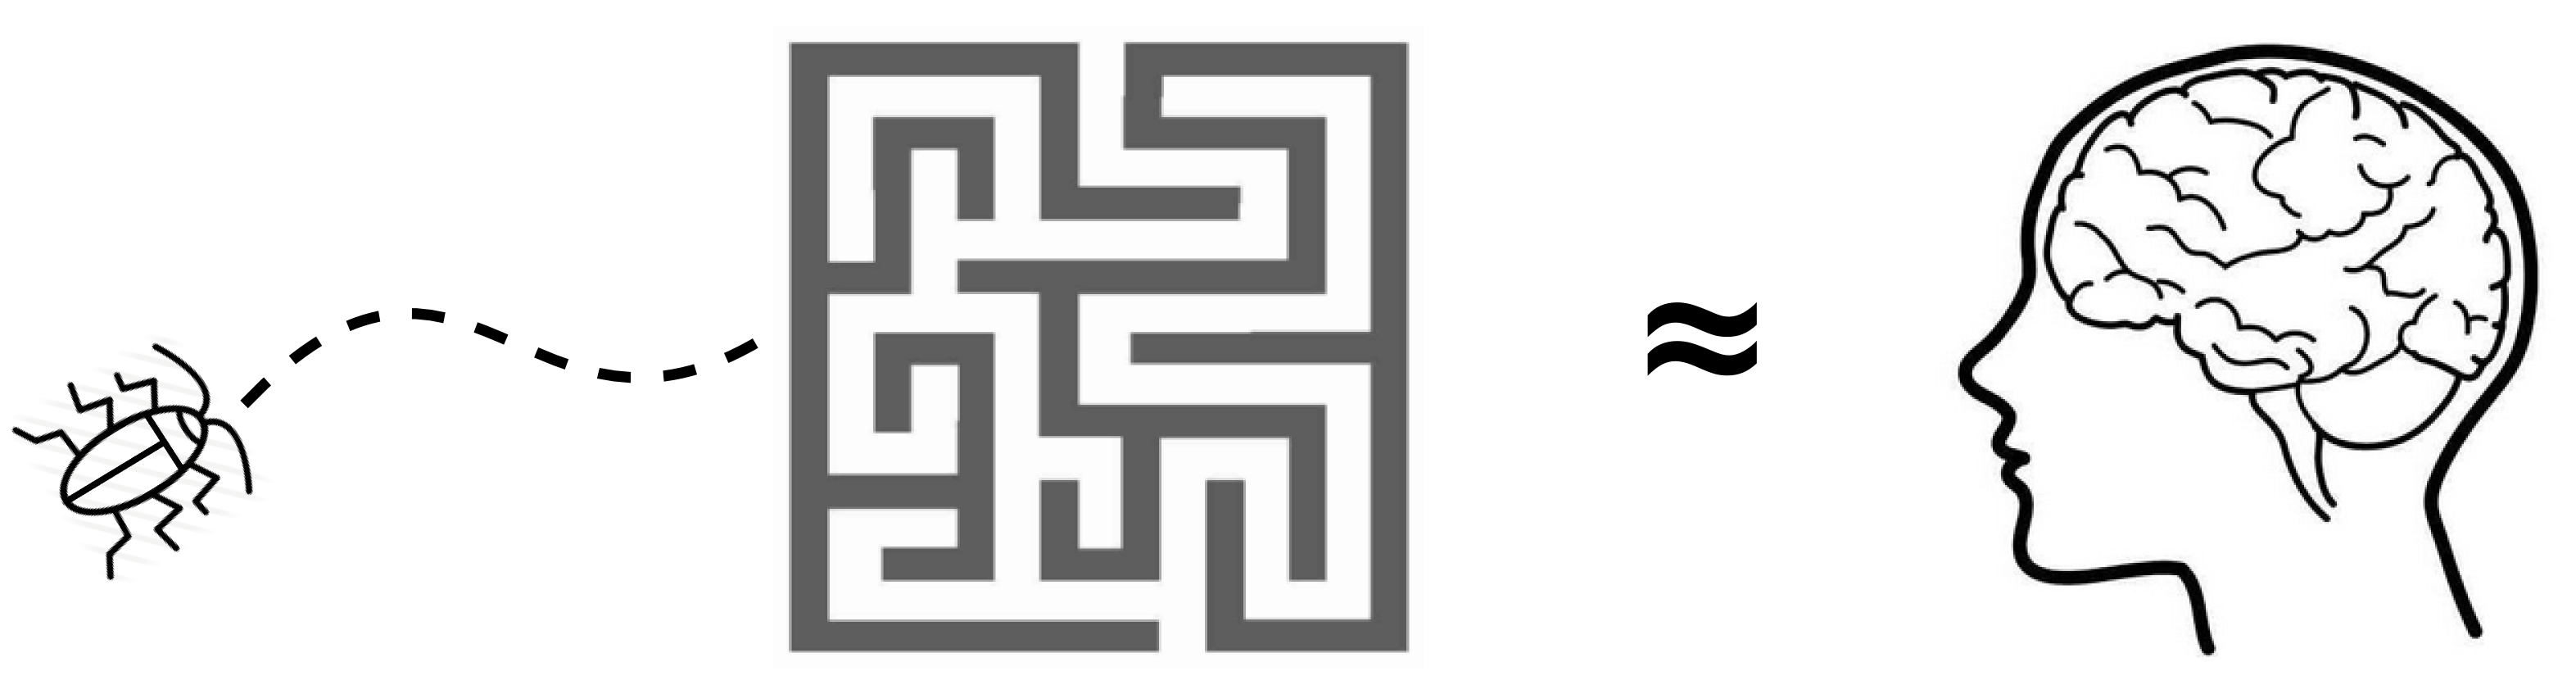
\includegraphics[scale=0.65]{maze-metaphor.png}
\end{equation}

关键是将「思考」看成是一个\emp{动态系统} (dynamical system),它运行在\emp{思维状态} (mental states) 的空间中:
\begin{equation}
\label{fig:mental-state}
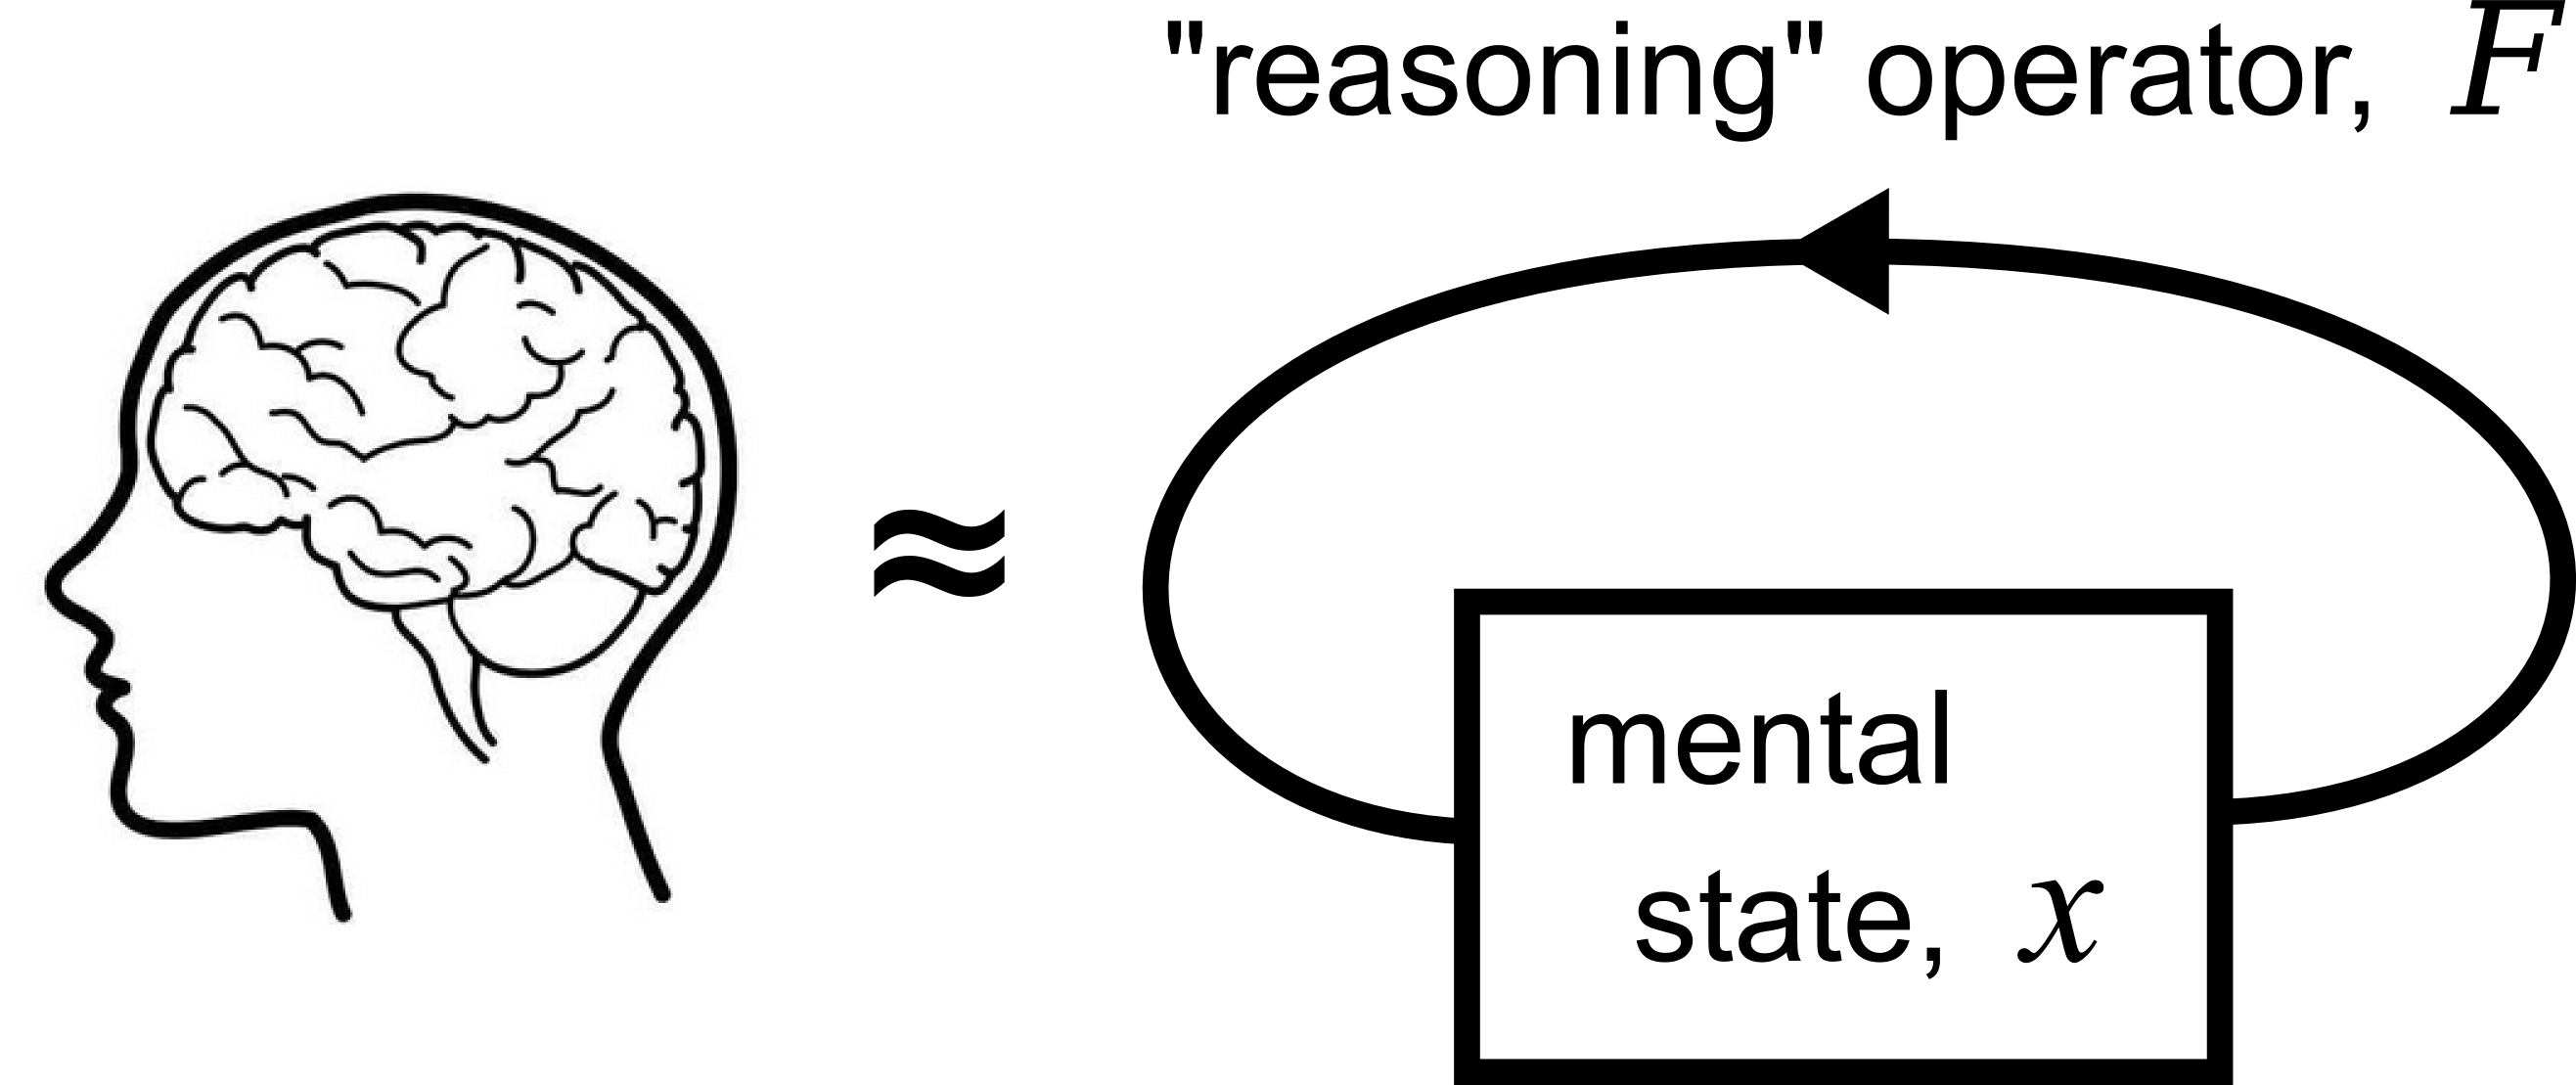
\includegraphics[scale=0.65]{mental-state.png}
\end{equation}

举例来说,一个\emp{思维状态}可以是以下的一束命题:
\let\labelitemi\labelitemii
\begin{itemize}
\item 我在我的房间内,正在写一篇 AGI-16 的论文。
\item 我正在写一句句子的开头:「举例来说,....」
\item 我将会写一个 NP (noun phrase):「一个思维状态....」
\end{itemize}

思考的过程就是从一个思维状态 \emp{过渡} (transition) 到另一个思维状态。 就算我现在说话,我的脑子也是靠思维状态记住我说话说到句子结构的哪部分,所以我才能组织句子的语法。

思维状态是一支向量 $\vect{x} \in X$,$X$ 是所有可能的思维状态,思考算子 (reasoning operator) $\vect{F}$ 是一个 endomorphism 映射: $X \rightarrow X$。

在数学上这是一个标准的\emp{动态系统 (dynamical system)},它可以用以下方法定义:
\begin{eqnarray}
\mbox{离散时间:} \quad \quad & \vect{x}_{t+1} = \vect{F}(\vect{x}_t) \\
\mbox{连续时间:} \quad \quad & \dot{\vect{x}} = \vect{f}(\vect{x}) \label{eqn1}
\end{eqnarray}

强化学习 (reinforcement learning)、动态规划 (dynamic programming)、控制论 (control theory) 的状态空间表述 ~ 三者其实是同义词; 在人工智能里习惯叫 RL。

%, we would have at disposal all the tools available in vector space such as:

%\begin{itemize}
%\item numerical optimization (including gradient descent)
%\item differential equations governing time evolution
%\item dynamical systems theory, control theory (eg. adaptive filters)
%\item Lie algebra and $C^*$-algebra of continuous operators
%\item matrix theory, iteration and fixed-point theory
%\item dynamic programming (aka. reinforcement learning)
%\item neural networks and deep learning ... etc.
%\end{itemize}

换句话说: 我们将逻辑 AI 的整套器材搬到向量空间中去实现。 这个做法,部分是受到 Google 的 PageRank \cite{Page1999} 和 Word2Vec \cite{Mikolov2013} 算法的启发,因为它们都是在向量空间中运作,而且非常成功。 %, both exploit the efficiency of vector and matrix calculus.

\section{控制论}

%以下内容可以在一般「现代控制论」教科书中找到,例如:
\let\labelitemi\labelitemii
%\begin{itemize}
%\item Daniel Liberzon 2012: \textit{Calculus of variations and optimal control theory -- a concise introduction}
%\item 李国勇 2008: 《最优控制理论与应用》
%\item 张洪钺、王青 2005: 《最优控制理论与应用》
%\end{itemize}

一个\emp{动态系统 (dynamical system)} 可以用以下方法定义:
\begin{eqnarray}
\mbox{离散时间:} \quad \quad & \vect{x}_{t+1} = \vect{F}(\vect{x}_t) \\
\mbox{连续时间:} \quad \quad & \dot{\vect{x}} = \vect{f}(\vect{x}) \label{eqn1}
\end{eqnarray}
其中 $f$ 也可以随时间改变。 如果 $f$ 不依赖时间,则系统是 time-invariant (定常的),形式上如(\ref{eqn1}) 那种微分方程叫作 autonomous (自主的)。

在我的智能系统理论里,我把 $F$ 或 $f$ 设定成 RNN (recurrent neural network),即反馈式神经网络:
\begin{eqnarray}
\mbox{离散时间:} \quad \quad & \vect{x}_{t+1} = \boxed{\mbox{RNN}}(\vect{x}_t) \\
\mbox{连续时间:} \quad \quad & \dot{\vect{x}} = \boxed{\mbox{RNN}}(\vect{x})
\end{eqnarray}
这里 recurrent 指的是它不断重复作用在 $\vect{x}$ 之上,但实际上它是一个普通的前馈式 (feed-forward) 神经网络。 注意: 在抽象理论中,$f$ 和 $F$ 可以是任意函数,我把它们设计成 NN 只是众多可能的想法之一。 之所以选用 NN,是因为它有 universal function approximator 的功能,而且是我们所知的最「聪明」的学习机器之一。

% Itamar Arel 在 2012 年提出的 \cite{Arel2012}

在我提出的智能系统里,$\dot{x}$ 是由\emp{學習機器}給出的,換句話說,$\dot{x}$ 是思維狀態在梯度下降至最佳狀態時的\emp{方向導數}。

一个(连续时间的)\emp{控制系统 (control system)} 定义为:
\begin{equation}
\dot{\vect{x}}(t) = f(\vect{x}(t), \vect{u}(t), t)
\end{equation}
其中 $\vect{u}(t)$ 是\emp{控制向量}。 控制论的目的就是找出最好的 $\vect{u}(t)$ 函数,令系统由初始状态 $\vect{x}_0$ 去到终点状态 $\vect{x_\bot}$。

注意: 人工智能中的 \emp{A* search},是动态规划的一个特例。 换句话说,用动态规划在某个空间中「漫游」,可以模拟到 best-first 搜寻的功能。

在这框架下,智能系统的运作可以分开成两方面: \emp{思考} 和 \emp{学习}。

\emp{思考}即是根据已学得的知识(知识储存在 RNN 里),在思维空间中找寻 $\vect{x}$ 最优的轨迹,方法是用控制论计算 $\vect{u}^*$。 $\vect{x}$ 的轨迹受 RNN 约束(系统只能依据「正确」的知识去思考),但思考时 RNN 是不变的。

\emp{学习}就是学习神经网络 RNN 的 weights $W$。 此时令 $u = 0$,即忽略控制论方面。

以上两者是两个独立的方面,但不排除它们可以在实际中同时进行。

\section{什么是强化学习?}

Reinforcement learning 是机器学习里面的一个分支,特别善於控制一只能够在某个环境下 \emp{自主行动} 的个体 (autonomous agent),透过和 \emp{环境} 之间的互动,例如 sensory perception 和 rewards,而不断改进它的 \emp{行为}。

听到强化学习,你脑里应该浮现一只曱甴那样的小昆虫,那就是 autonomous agent 的形象:
\begin{equation}

\includegraphics[scale=0.2]{cockroach.png}
\end{equation}

对「环境」(environment) 这概念,你应该想到像以下这经典游戏的迷宫:
\begin{equation}
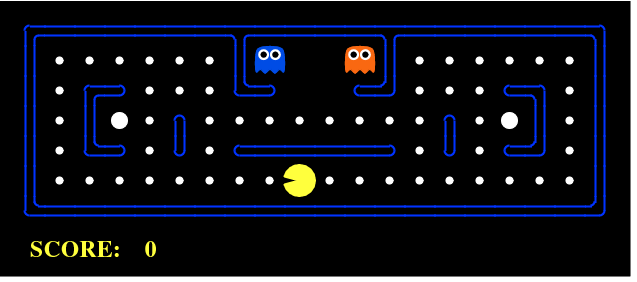
\includegraphics[scale=0.8]{pacman-0.png}
\end{equation}

包括有追捕你的怪物、和吃了会加分的食物 (这些代表负值和正值的 rewards)。  当然,实际应用的「环境」和「奖励」可以是抽象的,这游戏是一个很具体的例子。

\subsection{输入/输出}

记住,reinforcement learning 的 \emp{输入} 是:
\begin{itemize}
\item 状态 (States) = 环境,例如迷宫的每一格是一个 state
\item 动作 (Actions) = 在每个状态下,有什么行动是容许的
\item 奖励 (Rewards) = 进入每个状态时,能带来正面或负面的 价值 (utility)
\end{itemize}
而输出就是:
\begin{itemize}
\item 方案 (Policy) = 在每个状态下,你会选择哪个行动?
\end{itemize}
於是这 4 个元素的 tuple $(S,A,R,P)$ 就构成了一个强化学习的系统。   在抽象代数中我们常常用这 tuple 的方法去定义系统或结构。

再详细一点的例子就是:
\begin{itemize}
\item states $S$ = 迷宫中每一格的位置,可以用一对座标表示,例如 (1,3)
\item actions $A$ = 在迷宫中每一格,你可以行走的方向,例如: $\{$ 上,下,左,右 $\}$
\item rewards $R$ = 当前的状态 (current state) 之下,迷宫中的那格可能有食物 (+1) 、也可能有怪兽 (-100)
\item policy $P$ = 一个由 状态 $\rightarrow$ 行动 的 函数,意即: 这函数对给定的每一个状态,都会给出一个行动。 
\end{itemize}
$(S, A, R)$ 是使用者设定的, $P$ 是算法自动计算出来的。  

\subsection{人与虫之间}

第一个想到的问题是: 为什么不用这个方法打造人工智能?  但现时的强化学习算法,只对比较细小和简单的环境适用,对於大的复杂的世界,例如象棋的 $10^{\mbox{xxx}}$ 状态空间,仍是 intractable 的。

关键就是,高等智慧生物会在脑中建立世界的模型 (world model) 或知识 (knowledge), 而强化学习只是关心简单的「状态-行动」配对。

强化学习的领导研究者 Richard Sutton 认为,只有这种学习法才考虑到 自主个体、环境、奖励 等因素,所以它是人工智能中最 top-level 的 architecture,而其他人工智能的子系统,例如 logic 或 pattern recognition,都应该在它的控制之下,我觉得颇合理。
\begin{equation}
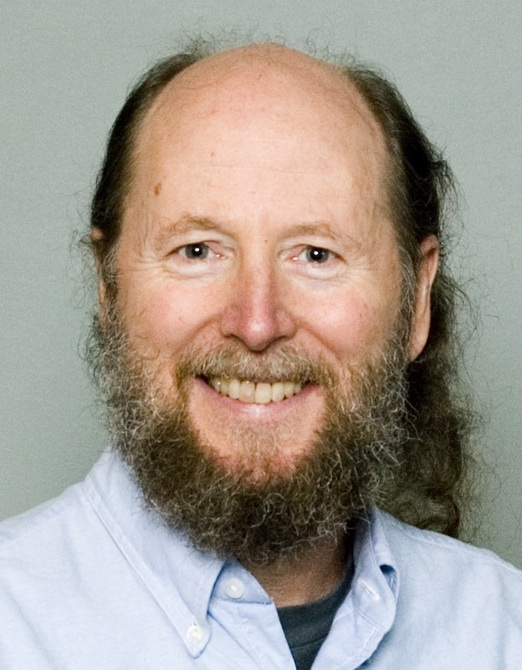
\includegraphics[scale=0.5]{Richard-Sutton.jpg}
\end{equation}

所以要制造 strong AI,一个可能的方案就是结合强化学习和某种处理复杂 world model 的能力:
\begin{equation}
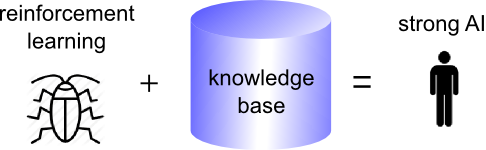
\includegraphics[scale=0.6]{cockroach-KB-person.png}
\end{equation}

\noindent 「\textit{你们已经由虫进化成人,但在你们之内大部份仍是虫。}」

\hfill --- 尼采, Thus spoke Zarathustra

\noindent 「\textit{如果人类不相信他们有一天会变成神,他们就肯定会变成虫。}」

\hfill --- Henry Miller

\begin{comment}
% ===========================================================================
\subsection{程式}

学 AI 最紧要有 program,不然就会很枯燥。  这是我在网上找到的一个特别简单的 demo,作者是 Travis DeWolf:

\href{https://studywolf.wordpress.com/2012/11/25/reinforcement-learning-q-learning-and-exploration/}{Reinforcement learning demo}

只要 Python 便可运行,但你可能要 install PyGame。

猫、老鼠、芝士:
\begin{equation}
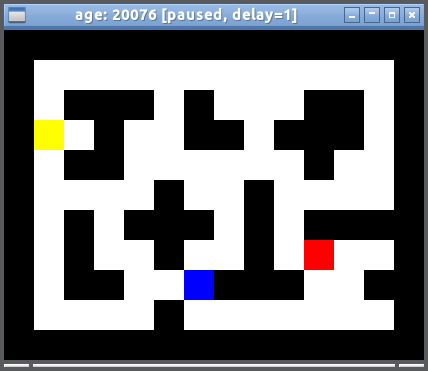
\includegraphics[scale=0.25]{RL-demo.png}
\end{equation}

猫的行动是简单地朝着老鼠追(没有智能),老鼠的行动是学习出来的。

注意,在 main program 和 cellular.py 这两部分,纯粹是定义了迷宫世界如何运作,基本上是一个 game,里面完全没有智能,你可以用{上、下、左、右} 控制各 agent 的活动,如此而已。

强化学习的程式在 qlearn.py,很短,而真正学习的程式基本上只有一句,就是:

\tab \code{def learnQ(self, state, action, reward, value): }\\
\tab \code{oldv = self.q.get((state, action), None) }\\
\tab \code{if oldv is None:} \\
\tab \code{\tab self.q[(state, action)] = reward }\\
\tab \code{else: }\\
\tab \code{\tab \textcolor{red}{self.q[(state, action)] = oldv + self.alpha * (value - oldv) }}

单是这一句程式,就能令老鼠学到避开猫、吃芝士。  以下再解释....

% ===========================================================================
\end{comment}

\subsection{強化學習的原理}

《AI-a modern approach》这本书第 21 章有很好的简介。  《AIMA》自然是经典,很多人说他们是读这本书而爱上 AI 的。  这本书好处是,用文字很耐性地解释所有概念和原理,思路很清晰,使读者不致有杂乱无章的感觉。  例如 21 章 首先讲 passive reinforcement learning,意思是当 policy 是固定时,纯粹计算一下 agent 期望的价值(utility,即 rewards 的总和) 会是多少。  有了这基础后再比较不同 policies 的好坏。  这种思路在数学中很常见: 首先考虑简单到连白痴也可以解决的 case,然后逐步引入更多的复杂性。  例如数学归纳法,由 $N=1$ 的 case 推到 $N \rightarrow \infty$。

为免重复,我只解释到明白 $Q$ learning 的最少知识。

\subsection{Utility (价值,或效)}

$U$ 是一连串行动的 rewards 的总和。  例如说,行一步棋的效用,不单是那步棋当前的利益,还包括走那步棋之后带来的后果。  例如,当下贪吃一只卒,但 10 步后可能被将死。  又或者,眼前有美味的食物,但有些人选择不吃,因为怕吃了会变肥。

一个 state 的效用 U 就是: 假设方案固定,考虑到未来所有可能的 transitions,从这个 state 开始的平均期望的 total reward 是多少 :

$$ U(S_0) = \mathbb{E}[ \; \sum_{t=0}^{\infty} \; \gamma^t \; R(S_t) \; ] $$

其中 $\mathbb{E[\;]}$ 代表期望值,$\gamma$ 是 discount factor,例如 0.9 或什么。

实例: 考虑这简单的迷宫:
\begin{equation}
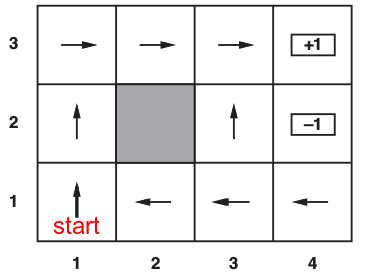
\includegraphics[scale=0.4]{RL-simple-maze.png}
\end{equation}

那些箭咀表示的是众多可能方案中的其中一个。

根据这个方案,由 $(1, 1)$ 开始的运行可能是这个结果:
\begin{equation}
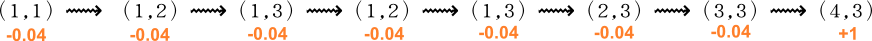
\includegraphics[scale=0.7]{RL-state-transition-eg-1.png}
\end{equation}

下面橙色的值是每个 state 的 reward。  在这例子中,每个不是终点的格,也会扣 0.04 分。

但从同一起点,同一方案,也可以出现不同结果,例如在 (1,3) 企图向右爬,但实际结果是向下跌一格; 这些 state transitions 是由外在世界的机率决定的。  (例如某人读了大学文凭,但遇上经济不景,他的薪水未必能达到行动的预期效果。)

同一方案的运行结果可以是:
\begin{equation}
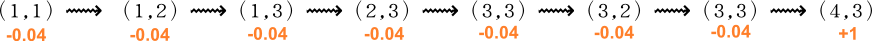
\includegraphics[scale=0.7]{RL-state-transition-eg-2.png}
\end{equation}
或者:
\begin{equation}
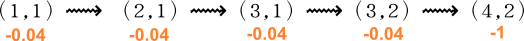
\includegraphics[scale=0.7]{RL-state-transition-eg-3.png}
\end{equation}

\subsection{Bellman condition}

这是 dynamic programming(动态规划)的中心思想,又叫 Bellman optimality condition。

在人工智能里我们叫 reinforcement learning,但在控制论的术语里叫 dynamic programming,两者其实是一样的。 Richard Bellman 在 1953 年提出这个方程,当时他在 RAND 公司工作,处理的是运筹学的问题。 他也首先使用了 "curse of dimensionality" 这个术语,形容动态规划的主要障碍。

考虑的问题是: 要做一连串的 sequential decisions。

Bellman equation 说的是: 「\textbf{如果从最佳选择的路径的末端截除一小部分,馀下的路径仍然是最佳路径。}」

换句话说,如果一系列的选择 A B C D E.... 是最优的,那么这系列除去开始的 A,那 B C D E.... 系列应用在后继的状态上也是最优的。

(例如,你从香港乘车到北京,选择了最便宜的路线,此路线经过 10 个车站,第二站是深圳:
$$ \mbox{香港} \rightarrow \mbox{深圳} \rightarrow ... ... \rightarrow \mbox{北京} $$
但如果除去出发点香港站,那么由第二站深圳到最后的北京站:
$$ \mbox{深圳} \rightarrow ... ... \rightarrow \mbox{北京} $$
这路线仍然是馀下 9 个站之间最便宜的。)

用数学表示:
$$ U^*(S) = \max_a \{ R(a) + U^*(S') \} $$
$$ U^*(\mbox{全路径}) = \max_a \{ R(\mbox{在当前状态下选取 a}) + U^*(馀下路径) \} $$
$*$ 表示 \emp{最优} (optimal)。 这条看似简单的式子是动态规划的全部内容; 它的意义是: 我们想获得最佳效益的路径,所以将路径切短一些,於是问题化解成一个较小的问题;  换句话说它是一个 recursive relation。

\subsection{Delta rule}

这只是一个简单的 trick,在机器学习中经常出现。  假设我们有一个理想,我们要逐步调教当前的状态,令它慢慢趋近这个理想。 方法是: 
$$ \mbox{当前状态} := \mbox{当前状态} + \alpha ( \mbox{理想} - \mbox{当前状态}) $$
其中 $\alpha$ 叫「学习速度 (learning rate)」。 "Delta" ($\Delta$) 指的是理想和现状之间的差异。

很明显,只要反覆执行上式,状态就会逐渐逼近理想值。

(Delta rule 的微分形式就是我们熟悉的「梯度下降」: $x \mbox{ += } \eta \cdot \frac{dy}{dx}$)

将 delta rule 应用到 Bellman condition 上,去寻找最优路径,这就是 Temporal Difference (TD) learning。

\begin{comment}
% ===========================================================================
\subsection{Temporal difference (TD) learning}

将 delta rule 应用到 Bellman condition 上,去寻找最优路径,这就是 temporal difference learning。

我们还是从简单情况开始:  假设方案固定,目标是学习每个 state 的 utility。

理想的 $U(S)$ 值,是要从 state $S$ 开始,试验所有可能的 transitions,再计算这些路径的 total rewards 的平均值。

但实际上,agent 只能够每次体验一个行动之后的 state transition。

所以要应用 Bellman condition: 一个 state $S$ 的 $U$ 值,是它自身的 reward,加上所有可能的后继 states 的 $U$ 值,取其机率平均,再乘以 discount factor $\gamma$:
$$ U(S) = R(S) + \gamma \sum_{S'} P(S \rightarrow S') \; U(S') $$
其中 $P$ 是 transition 的机率,$S'$ 是后继 state,$\sum$ 是对所有后继 states 求和。  换句话说,这是理想的 $U(S)$ 和 $U(S \mbox{的后继})$ 之间的关系,是一个 recursive relation。

例如,假设 agent 现时对 state (1,3) 和 state (2,3) 的估值,分别为 0.84 和 0.92。  又假设 agent 察觉到,根据现有方案,在 (1,3) 时总是会发生跳到 (2,3) 这个 transition。  那么这两个 states 的 $U$ 值,应该符合这条约束:
$$ U(1,3) = -0.04 + U(2,3) $$
换句话说,这是两个 states 之间,U 值的 local (局部的)约束。

TD learning 的思想是:  假设其他 $U(S')$ 的值正确,利用 Bellman optimality 来调整当下 state 的 $U(S)$。 当尝试的次数多了,所有 $U$ 值都会趋向理想。 Agent 只需要用这条 update rule:
$$ U(S) \mbox{  +=  } \alpha ( \; R(S) + \gamma U(S') - U(S) \; ) $$

$\alpha$ 是 learning rate,它决定学习的速度(但它不能太大,避免 overshooting)。  后面那东西是 $U(S)$ 和 $U(S)$ 的估值 (estimation) 之间的差别。  对於理想的 $U(S)$ 和 $U(S')$,那差别会是 0。  而在每个 time step,我们只是用 $\alpha$ 部分地 调整这个差别。

最后一提,在上面理想约束的公式里,有对於机率 P 的求和,但在 update formula 中 $P$ 不见了。  那是因为 agent 在环境中的行动,暗含了对於 state transition 机率的 sampling (随机地取样本)。 换句话说,那机率求和是由 agent 本身体现的。

$P$ 是 state transitions 的机率,换句话是关於世界的一个 model。 TD learning 不需要学习 $P$,所以叫 model-free learning。  但正如开篇时说过,model-free 并不一定是好事,人的智慧就是基於我们对外在世界有一些很好的 models。

\end{comment}
% ===========================================================================

\subsection{Q value}

$Q$ 值只是 $U$ 值的一个变种 ;   $U$ 是对每个 state 而言的,$Q$ 把 $U$ 值分拆成每个 state 中的每个 action 的份量。  换句话说,$Q$ 就是在 state $S$ 做 action $A$ 的 utility。

$Q$ 和 $U$ 之间的关系是:
$$ U(S) = \max_A  Q(A, S) $$

$Q$ 的好处是什么?  下面将会介绍 active learning,而 $Q$ value  配合 TD learning,可以在 active learning 中也消除 $P$,达到 model-free 的效果。

上面的 update rule 只要用这个关系改写就行:
$$ U(S) \mbox{  +=  } \alpha ( \; R(S) + \gamma \max_{A'}  Q(A', S') - Q(A, S) \; ) $$

\begin{comment}
% ===========================================================================
\subsection{Active learning}

在 passive learning 中,方案不变,我们已经能够计算每个 state $S$ 的效用 $U(S)$,或者每个 state $S$ 之下行动 $A$ 的效用 $Q(S, A)$。

如果方案是可以改变的,我们只需计算不同方案的 $Q$ 值,然后在每个 state $S$ 选取相应於最大 $Q$ 值的行动 $A$,那就是最佳方案,不是吗?

实际上执行的结果,却发现这些 agent 的方案很差!  原因是,学习过程中的 $Q$ 值是 estimate,不是理想的 $Q$ 值,而如果根据这样的 $Q$ 行动,agent 变得很短视,不会找到 optimal policy。  (例如,某人经常吃同一间餐馆,但循另一路径走,可以发现更好的餐馆。)

Agent 需要尝试一些未知的状态/行动,才会学到 optimal policy;  这就是所谓的 exploration vs exploitation (好奇心 vs 短暂贪婪)之间的平衡。

方法是,人工地将未知状态的价值增加一点:
$$ U(S) = R(S) + \gamma \max_A \mathcal{F}[ \; \sum_{S'} P(S \rightarrow S') U(S'), \; N(A, S) \; ] $$
其中 $N(A, S)$ 是状态 $S$ 和行动 $A$ 这对组合出现过(被经历过)的次数,$\mathcal{F}$ 是 exploration 函数,它平时回覆正常的 $U$ 的估计值,但当 $N$ 很小时(亦即我们对 $S$,$A$ 的经验少),它会回覆一个比较大的估值,那代表「好奇心」的效用。

% 结语

% 本来想写一篇人人能读懂的 RL 简介,但发觉写到长篇大论才勉强解释完。  希望女朋友能读懂 :)
\end{comment}
% ===========================================================================

\section{控制论}

在\emp{强化学习}中,我们关注两个数量:
\let\labelitemi\labelitemii
\begin{itemize}
\item $R(\vect{x},a)$ = 在状态 $\vect{x}$ 做动作 a 所获得的\emp{奖励}(reward)
\item $U(\vect{x})$ = 状态 $\vect{x}$ 的\emp{效用}(utility) 或 \emp{价值} (value) % 或 $V(\vect{x})$
\end{itemize}
简单来说,「价值」就是每个瞬时「奖励」对时间的积分:
\begin{equation}
\boxed{\mbox{价值} U} = \int \boxed{\mbox{奖励} R} \,dt
\end{equation}
(价值有时用 $V$ 表示,但为避免和势能 $V$ 混淆故不用。)

用\emp{控制论}的术语,通常定义 cost functional:
\begin{equation}
J = \int L dt + \Phi(\vect{x}_\bot)
\end{equation}
其中 $L$ 是 ``running cost'',即行走每一步的「价钱」; $\Phi$ 是 terminal cost,即到达终点 $\vect{x}_\bot$ 时,那位置的价值。

%Define a continuous version of ``utility'':
%\begin{equation}
%V(x,t) = \min_u \{ \int_t^{t_\bot} C(x,u)dt + \Phi(x_\bot,t_\bot) \} 
%\end{equation}
%where $t$ is time, $u$ is a set of control parameters, $C$ is the \emp{cost-rate} function:
%\begin{equation}
%\int C dt = R = \mbox{reward}
%\end{equation}
%This integral expresses the ``cost of the path'', whereas $\Phi(x_\bot,t_\bot)$ is the ``cost at termination''.

在\emp{分析力学}里 $L$ 又叫 Lagrangian,而 L 对时间的积分叫「作用量」:
\begin{equation}
\boxed{\mbox{作用量 (Action) \; S}} = \int L dt
\end{equation}
Hamilton 的\emp{最小作用量原理} (principle of least action) 说,在自然界的运动轨迹里,$S$ 的值总是取稳定值 (stationary value),即比起邻近的轨迹它的 $S$ 值最小。

所以有这些对应:
\begin{center}
\begin{tabular}{|c|c|c|}
\hline 
\emp{强化学习} & \emp{最优控制} & \emp{分析力学} \\ 
\hline
效用/价值 $U$ & 价钱 $J$ & 作用量 $S$ \\ 
\hline 
即时奖励 $R$ & running cost & Lagrangian $L$ \\ 
\hline 
action $a$ & control $u$ & (外力?) \\
\hline
\end{tabular} 
\end{center}

用比较浅显的例子: 和美女做爱能带来即时的快感 (= 奖励 $R$),但如果强奸的话会坐牢,之后很长时间很苦闷,所以这个做法的长远价值 $U$ 比其他做法较低,正常人不会选择它。

有趣的是,奖励 $R$ 对应於力学上的 Lagrangian,其物理学单位是「能量」; 换句话说,「快感」或「开心」似乎可以用「能量」的单位来量度,这和通俗心理学里常说的「正能量」不谋而合。 而,长远的价值,是以 $[\mbox{能量} \times \mbox{时间}]$ 的单位来量度。

一个智能系统,它有「智慧」的条件,就是每时每刻都不断追求「开心能量」或奖励 $R$ 的最大值,但它必需权衡轻重,有计划地找到长远的效用 $U$ 的最大值。

\begin{comment}
% ===========================================================================
\subsection{经典分析力学(analytical mechanics)}

分析力学的物理内容,完全是牛顿力学的 $F = ma$,但在表述上引入了能量和 Hamiltonian 等概念,再使用微积分和变分法。

\subsubsection{Lagrange 方程}

Lagrange 引入了 Lagrangian $L = T - V$,可以分拆成\emp{動能} $T$ 和\emp{勢能} $V$ 兩部分。

重點是: \emp{動能} $T$ 是速度 $\dot{\vect{x}}$ 的函數,\emp{勢能} $V$ 是位置 $\vect{x}$ 的函數。

问题: 如果在强化学习中的「快感/奖励」对应於 Lagrangian $L$,如何在奖励之中分拆出「动能」和「势能」的分量? 

\begin{equation}
\boxed{\mbox{Lagrange equation}} \quad
\frac{d}{dt} \frac{\partial L}{\partial \dot{x}_i} - \frac{\partial L}{\partial x_i} = 0
\end{equation}
这些方程的座标是 $(\vect{x}, \dot{\vect{x}})$,可以了解成\emp{位置空间 (configuration space)}上的 tangent bundle (下述)。

\subsubsection{Hamilton 方程}

\emp{Hamiltonian} $H = T + V$,亦即总能量,但它表示成位置 $\vect{x}$ 和动量 $\vect{p}$ 的函数。

\begin{equation}
\label{Hamilton-eqns}
  \boxed{\mbox{Hamilton equation}} \quad
  \begin{cases}
      \dot{\vect{x}} & = \displaystyle \frac{\partial H}{\partial p} \\
      \dot{\vect{p}} & = - \displaystyle \frac{\partial H}{\partial x}
  \end{cases}
\end{equation}
这些方程的座标是\emp{相位空间 (phase space)} $(\vect{x}, \vect{p})$。

位置空间和相位空间之间的变换是 \emp{Legendre transformation}:
\begin{eqnarray}
\boxed{\mbox{tangent bundle}} \; T X & \rightarrow & T^* X \; \boxed{\mbox{cotangent bundle}} \\
(\vect{x}, \dot{\vect{x}}) & \mapsto & (\vect{x}, \vect{p})
\end{eqnarray}
\begin{equation}
\vect{p} = \frac{\partial L}{\partial \dot{\vect{q}}} \quad \Rightarrow \quad H := \vect{p} \dot{\vect{x}} - L
\end{equation}

\subsubsection{Hamilton-Jacobi 方程}

\begin{equation}
\boxed{\mbox{Hamilton-Jacobi equation}} \quad
H(q, \frac{\partial S}{\partial q}, t) + \frac{\partial S}{\partial t} = 0
\end{equation}
其中 $S$ 是「作用量」。 下面我们会用动态规划的原理推导出此一方程。

\subsubsection{Poisson 括号}

\begin{equation}
\label{Poisson-bracket}
\boxed{\mbox{Poisson 括号}} \quad \{ F, H \} := \sum_i \{ \frac{\partial F}{\partial q_i} \frac{\partial H}{\partial p_i} - \frac{\partial F}{\partial p_i} \frac{\partial H}{\partial q_i} \}
\end{equation}
在力学系统中,它表示任意一力学量(函数 $f$)对时间的改变量:
\begin{equation}
\dot{f} = \{ f, H \} 
\end{equation}
\begin{equation}
\frac{\partial}{\partial t} = \frac{\partial}{\partial p} \dot{p} + \frac{\partial}{\partial q} \dot{q}
\end{equation}
以上使用了微分的 chain rule,但由於 $\dot{\vect{p}}$ 和 $\dot{\vect{q}}$ 可以由 Hamilton 方程 (\ref{Hamilton-eqns}) 给出,所以得到 Poisson 括号的形式 (\ref{Poisson-bracket})。

每个物理学生都知道的「经典-量子对应原理」:
\begin{equation}
[\vect{F}, \vect{G}] \quad \Leftrightarrow \quad i \hbar \{ F, G \}
\end{equation}
这对应原理是 P.A.M. Dirac 发现的。

在经典力学里,
\begin{equation}
\{ \vect{x}, \vect{p} \} = 1
\end{equation}
但在量子力学里,
\begin{equation}
[ \vect{X}, \vect{P} ] = i \hbar
\end{equation}
这也是 Heisenberg 测不准原理的由来:
\begin{equation}
\Delta \vect{X} \Delta \vect{P} \ge \frac{\hbar}{2}
\end{equation}

如果在某一流形上,「广义」Poisson 括号是 nondegenerate (非退化)的,则它变成了\emp{辛流形}结构的 $\omega = \{ \cdot, \cdot \}$ 括号 (下述)。

\subsection{Hamiltonian 的出现}

考虑一个典型的控制论问题,系统是:
\begin{eqnarray}
\mbox{状态方程:} \quad & \dot{\vect{x}}(t) = \vect{f}[\vect{x}(t), \vect{u}(t), t] \\
\mbox{边值条件:} \quad & \vect{x}(t_0) = \vect{x}_0 \,,\, \vect{x}(t_\bot) = \vect{x}_\bot \\
\mbox{目標函数:} \quad & J = \int_{t_0}^{t_\bot} L[\vect{x}(t), \vect{u}(t), t] dt
\end{eqnarray}
要找的是最优控制 $\vect{u}^*(t)$。

\begin{figure}[H]
\begin{center}
\colorbox{grey}{\parbox{0.95\textwidth}{\setlength{\parskip}{2.5ex}

\emp{Lagrange multiplier} 是找极大/小值的常用方法: 如果我们要找:
\begin{equation}
\max \; f(x) \quad \mbox{ subject to } \quad g(x) = 0
\end{equation}
Lagrange 建议我们建构 Lagrangian 函数:
\begin{equation}
L(x, \lambda) = f(x) - \lambda g(x)
\end{equation}
然后求解:
\begin{equation}
\nabla_{x,\lambda} L = 0
\end{equation}
}}
\end{center}
\end{figure}

现在将 Lagrange multiplier 方法应用到我们的问题上,会发现新的目标函数是:
\begin{equation}
J = \int_{t_0}^{t_\bot} \{ L + \vect{\lambda}^T(t) \left[ f(\vect{x}, \vect{u}, t) - \dot{\vect{x}} \right] \} dt
\end{equation}
因此可以引入一个新的标量函数 $H$,即 Hamiltonian:
\begin{equation}
H(\vect{x}, \vect{u}, t) = L(\vect{x}, \vect{u}, t) + \vect{\lambda}^T(t) f(\vect{x}, \vect{u}, t)
\end{equation}
物理学上,$\vect{f}$ 的单位是速度,而 $L$ 的单位是能量,所以 $\vect{\lambda}$ 应该具有 \emp{动量} 的单位。

\subsubsection{极小值原理}

Lev Pontryagin (1908-1988) 提出了 \emp{极小值原理},是经典变分法的推广。 经典变分法的最优条件是:
\begin{equation}
\frac{\partial H}{\partial \vect{u}} = \vect{0}
\end{equation}
极小值原理将最优条件改成是:
\begin{equation}
\min_{u \in \Omega} H(\vect{x}^*, \vect{\lambda}^*, \vect{u}, t) = H(\vect{x}^*, \vect{\lambda}^*, \vect{u}^*, t)
\end{equation}
即是说: 在最优轨迹 $\vect{x}^*(t)$ 和最优控制 $\vect{u}^*(t)$ 上,$H$ 取最小值。 它的好处是,当 $\displaystyle \frac{\partial H}{\partial \vect{u}}$ 不连续或不存在时,或者 $\vect{u}$ 受其他约束时,也可以应用。

粗略来说,极小值原理比经典变分法更一般,而动态学习又比极小值原理更一般。

\subsubsection{Hamilton-Jacobi-Bellman 方程}

\begin{itemize}
\item Stanislaw Zak (2003): \textit{Systems and control}
\end{itemize}

% \S 5.4.3 Zak.

用动态规划的 \emp{Bellman optimality condition} 可以推导出微分形式的 Hamilton-Jacobi-Bellman 方程。  重温一下,Bellman 最优条件说的是: 「从最优路径末端切去一小截之后,馀下的还是最优路径。」  它通常写成如下的 recursive 形式:
\begin{eqnarray}
\boxed{\mbox{最优路径}} & = & \mbox{在小段上选取最大奖励} + \boxed{\mbox{馀下的最优路径}} \\
J^*_t & = & \max_{u} \{ \boxed{\mbox{奖励}(u, t)} + J^*_{t-1} \}
\end{eqnarray}

\begin{equation}
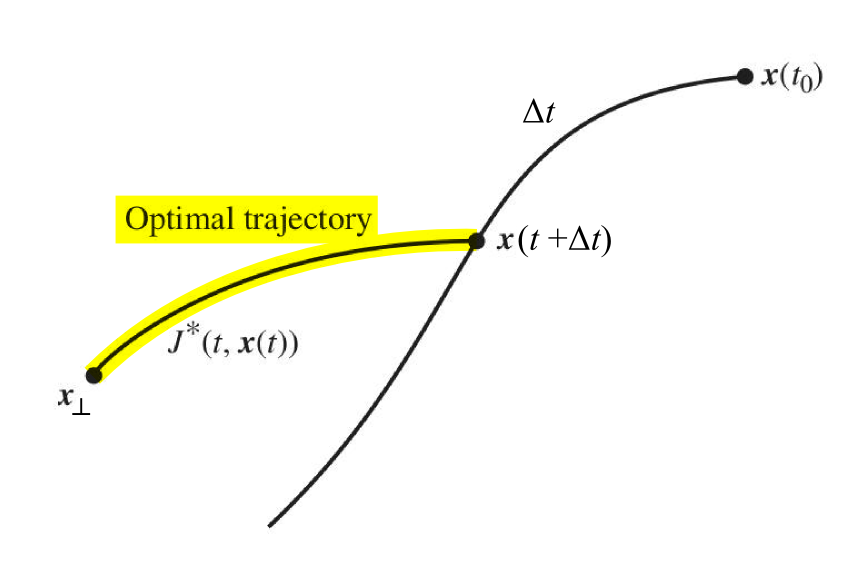
\includegraphics[scale=0.4]{optimal-trajectory.png}
\end{equation}

我们在时间 interval 的开端切出一小段:
\begin{equation}
[ t_0, t_\bot ] = [ t_0, t_0 + \Delta t ] \cup [ t_0 + \Delta t, t_\bot ]
\end{equation}
我们想优化的目标函数是:
\begin{equation}
J^*(t, \vect{x}, \vect{u}) = \min_u \{ \int_{t_0}^{t + \Delta t} L d\tau + \int_{t + \Delta t}^{t_\bot} L d\tau + \Phi(t_\bot, \vect{x}_\bot) \}
\end{equation}
根据 Bellman 条件,目标函数变成:
\begin{equation}
J^*(t, \vect{x}) = \min_u \{ \int_{t_0}^{t + \Delta t} L d\tau + J^*(t + \Delta t, \vect{x}(t + \Delta t)) \}
\end{equation}
用 Taylor series 展开右面的 $J^*$:
\begin{equation}
J^* + \frac{\partial J^*}{\partial t} \Delta t + \frac{\partial J^*}{\partial \vect{x}}(\vect{x}(t + \Delta t) - \vect{x}(t)) + \mbox{H.O.T.}
\end{equation}
左右两边的 $J^*$ 互相消去,而且 $\vect{x}(t + \Delta t) - \vect{x}(t) \approx \dot{\vect{x}} \Delta t$,於是有:
\begin{equation}
0 = \min_u \{ \int_{t_0}^{t + \Delta t} L d\tau + \frac{\partial J^*}{\partial t} \Delta t + \frac{\partial J^*}{\partial \vect{x}} \dot{\vect{x}} \Delta t + \mbox{H.O.T.} \}
\end{equation}
又由於 $\Delta t$ 很小,而且 $\dot{\vect{x}} = \vect{f}$,所以:
\begin{equation}
0 = \min_u \{ L \Delta t + \frac{\partial J^*}{\partial t} \Delta t + \frac{\partial J^*}{\partial \vect{x}} \vect{f} \Delta t + \mbox{H.O.T.} \}
\end{equation}
全式除以 $\Delta t$ 并令 $\Delta t \rightarrow 0$:
\begin{equation}
0 = \frac{\partial J^*}{\partial t} + \min_u \{ L + \frac{\partial J^*}{\partial \vect{x}} \vect{f} \}
\end{equation}
记得 Hamiltonian 的定义是 $\displaystyle H = L + \frac{\partial J^*}{\partial \vect{x}} \vect{f}$,所以得到想要的结果:
\begin{equation}
\boxed{\mbox{Hamilton-Jacobi equation}} \quad
0 = \frac{\partial J^*}{\partial t} + \min_u H
\end{equation}

% The differential version is the Hamilton-Jacobi equation:
% \begin{equation}
% \frac{d}{dt} V(x,t) = \min_u \{ C(x,u) + \langle \nabla V(x,t), f(x,u) \rangle \} 
% \end{equation}
% where $x$ must obey this dynamics:
% \begin{equation}
% \dot{x}(t) = f(x(t),u(t)).
% \end{equation}

这个方程和量子力学中的 \emp{Schr\"{o}dinger equation} 很相似:
\begin{equation}
i \hbar \frac{\partial}{\partial t} \Psi(x,t) = \left[ V(x,t) + \frac{-\hbar^2}{2\mu} \nabla^2 \right] \Psi(x,t).
\end{equation}
其中 $\Psi$ 类似於我们的 $J$ (或许 $\Psi$ 是自然界希望取极值的某种东西?)

\subsection{Symplectic 结构}

\begin{itemize}
\item Stephanie Singer (2001): \textit{Symmetry in mechanics -- a gentle, modern introduction}
\item 锺万勰 2011: 《力、功、能量与辛数学》
\end{itemize}

Symplectic 的拉丁文意思是「互相交错 (intertwined)」,它用来描述 Hamiltonian 系统的几何结构。 中文译作「辛」是音译。  Symplectic 概念是 Hermann Weyl 研究 Hamilton 系统的对称性时在 1939 年提出的。

在数值计算上,处理 Hamilton 系统时,如果算法尊重 symplectic 结构(叫 symplectic integrators),会比一般的算法更准确; 而一般解微分方程的算法,例如 Euler 算法和 Runge-Kutta 算法,有时会给出错误的结果。

举例来说,从 Hamiltonian 的角度来看,动量 $p$ (momentum) 和 速度 $v$ (velocity) 是成\emp{对偶}的,$p$ 总是伴随 $v$ 出现,因为 $p \cdot v = mv^2$ 的单位是能量。

举另一个例子,假设我们有两个用来定义系统状态的向量:
\begin{equation}
x_1 = \left(
\begin{array}{c}
s_1\\
f_1\\
\end{array}
\right), \quad
x_2 = \left(
\begin{array}{c}
s_2\\
f_2\\
\end{array}
\right)
\end{equation}
其中 $s$ 是位移(单位是长度),$f$ 是力。 这两个向量的「辛内积」定义为:
\begin{eqnarray}
\langle x_1, x_2 \rangle & = & x_1^T \, J \, x_2 \nonumber \\
& = &
\left(
\begin{array}{c}
s_1\\
f_1\\
\end{array}
\right)^T
\left( \begin{array}{cc}
0  & I \\
-I & 0 \end{array} \right)
\left(
\begin{array}{c}
s_2\\
f_2\\
\end{array}
\right) \\
& = & f_2 s_1 - f_1 s_2 \nonumber
\end{eqnarray}
其中矩阵 $J$ 就是辛的微分形式 $\omega$ 的结构矩阵(下述)。 由於 $f \cdot s$ 表示的是「所做的功」,上式表示的是
\begin{multline}
(\mbox{状态1的力对状态2的位移所做的功}) - \\
(\mbox{状态2的力对状态1的位移所做的功})
\end{multline}
也就是「相互功」,辛正交则 $\langle x_1, x_2 \rangle = 0$,代表 work reciprocity(功的互等),所以辛几何是一种关於能量的代数。

在微分几何里,研究抽象的 Hamiltonian systems,会发现 symplectic 结构。 这结构用微分流形 $M$ 及其上的一个 微分形式 (differential form) $\omega$ 来定义。 需要一些微分几何的基础.....

\subsubsection{Vector fields, differential forms, Hamiltonian flow}

根据 Hamilton 方程,再用微分的 chain rule 可以得到:
\begin{equation}
\frac{d}{dt} = \frac{\partial H}{\partial \vect{p}} \frac{\partial}{\partial \vect{x}} - \frac{\partial H}{\partial \vect{x}} \frac{\partial}{\partial \vect{p}}
\end{equation}
它是一个微分算子,亦即是\emp{向量场}; 它有个特别的名字叫 Hamiltonian flow $\vec{H}$ (很多书记作 $X_H$):
\begin{equation}
\vec{H} := \frac{d}{dt} = \{ \cdot, H \}
\end{equation}
可以看出 $\vec{H} H = \{ H, H \} = \frac{dH}{dt} = 0$ 就是\emp{能量守恒}的形式。

Hamilton 系统的动态方程就是:
\begin{equation}
\dot{\vect{x}} = \vec{H}
\end{equation}
所以在我们的智能系统中,RNN 可以看成是 $\vec{H}$。

\begin{eqnarray}
\omega & = & \sum_i dx_i \wedge dp_i \\
\omega(\vec{H}, \cdot) & = & dH
\end{eqnarray}
我暂时不很明白它的意义。

我们说 Hamiltonian flow 保持 (preserve) 辛结构。 假设 $\Gamma_t(\vect{x}_0) = \vect{x}(t)$ 描述 Hamiltonian flow 的轨迹; $\Gamma_0(\vect{x}) \equiv \vect{x}$。 The \emp{pullback} of $\omega$ along $\Gamma$ is still $\omega$:
\begin{equation}
\Gamma^*_t \omega = \omega
\end{equation}
\begin{equation}
\vec{H} H = 0 \quad \mbox{is equivalent to} \quad \Gamma^*_t \omega = \omega
\end{equation}
\end{comment}
% ===========================================================================

\section{Episodic memory}

设计了这个 minimalist architecture 之后,发现比较起人脑有个严重缺陷,就是没有「事件记忆」(换句话说,只能留意当下发生的事件,但不能记住一段故事)。

这牵涉到甚么是「记忆」的问题。 在 minimal architecture 里,$\vect{F}$ 代表 ``static knowledge'',亦即(相对地)永恒不变的规律,而 $\vect{x}$ 代表当下的状态,亦即 ``dynamic knowledge''。

Episodic memory 介乎「动态」与「静态」之间,我估计和信息处理理论中的 $z$-transform 或许有关。 Episodic memory 的问题仍有待研究,但没有 episodic memory 也可以制造一种颇为有用的智能系统了。 

\section{经典逻辑 AI}

Strong AI 的问题在理论上已经被\emp{数理逻辑}完整地描述了,馀下的问题是\emp{学习算法},因为在逻辑 AI 的架构下,学习算法很慢(复杂性很高),这就是我们要解决的。

我研究 logic-based AI 很多年,因此我的思路喜欢将新问题还原到逻辑 AI 那边去理解,但实际上我提倡的解决办法不是靠经典逻辑,甚至不是 symbolic 的。  但在这篇文章我还是会经常跳回到逻辑 AI 去方便理解。

用数理逻辑模拟人的思想是可行的,例如有 deduction, abduction, induction 等这些模式,详细可见《Computational logic and human thinking》by Robert Kowalski, 2011.  这些方面不影响本文的阅读。 值得一提的是,作者 Kowalski 是 logic programming,特别是 Prolog,的理论奠基人之一。

在经典逻辑 AI 中,「思考」是透过一些类似以下的步骤:
\begin{eqnarray}
\mbox{前提} & \vdash & \mbox{结论} \\
\boxed{\mbox{今天早上下雨}} & \vdash & \boxed{\mbox{草地是湿的}}
\end{eqnarray}
亦即由一些\emp{命题}(propositions)推导到另一些命题。

推导必须依靠一些逻辑的法则命题 (rule propositions),所谓「法则」是指命题里面带有 x 这样的\emp{变量}(variables):
\begin{equation}
\boxed{\mbox{地方 x 下雨}} \wedge \boxed{\mbox{x 是露天的}} \vdash \boxed{\mbox{地方 x 是湿的}}
\end{equation}
这些法则好比「逻辑引擎」的燃料,没有燃料引擎是不能推动的。

注意: 命题里面的 x,好比是有「洞」的命题,它可以透过 substitution 代入一些实物 (objects),而变成完整的命题。 这种「句子内部」(sub-propositional)的结构可以用 predicate logic (谓词逻辑)表达,但暂时不需要理会这些细节。

Logic-based AI 可以看成是将世界的「模型」压缩成一个「知识库」(knowledge-base, KB),里面装著大量逻辑式子:
\begin{equation}
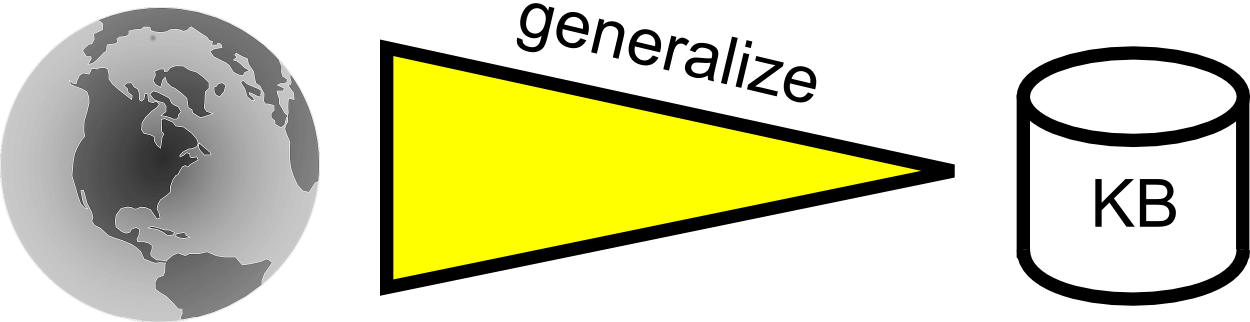
\includegraphics[scale=0.5]{world-model-compression.png}
\end{equation}
世界模型是由大量的逻辑式子经过组合而\emp{生成}的,有点像向量空间是由其「基底」生成; 但这生成过程在逻辑中特别复杂,所以符号逻辑具有很高的\emp{压缩比},但要学习一套逻辑知识库,则相应地也有极高的\emp{复杂度}。

\section*{Acknowledgements}

\footnotesize{In a forum discussion with Ben Goertzel dated 25 June 2014 on the AGI mailing-list: (artificial-general-intelligence @googlegroups.com), YKY asked: Why bother with neural networks, which typically require many neurons to encode data, when logic-based AI can represent a proposition with just a few symbols?  Ben's insight is that neural networks are capable of learning its own representations, and their learning algorithms are relatively fast.  We have been working on "neo-classical" logic-based AI for a long time, and begin to realize that inductive learning in logic (based on combinatorial search in a symbolic space) is perhaps \textit{the bottleneck} in the entire logic-based paradigm.  So we try to look for alternatives that might enable learning to be faster, though we would still emphasize that logic-based AI remains a viable approach to AGI. %, provided that the right search heuristics be found (most probably in the form of \emp{hierarchical organization} of the learning space).
}

\bibliographystyle{plain} % or number or aaai ...
\bibliography{AGI-book}

\end{document}
